\setchapterstyle{kao}
\setchapterpreamble[u]{\margintoc}
\chapter{Linguistic factors used as predictors}
\labch{predictors}

This Chapter presents the five linguistic factors I will use as predictors in my Stochastic OT model of implicit indefinite objects, defined in \nrefch{modeltheory}. The theory linking each of these factors to the omissibility of direct objects is discussed at length in \nrefch{factors}.


\section{Recoverability} \labsec{predictor_sps}

% MEDINA PDF 32, aggiungere al mio paragrafo/capitolo su PISA!

%  In brief, these qualities include not stipulating verb meaning or selectional preferences but rather modeling a verb’s selection of argument classes in terms of production data, quantifying what a speaker knows about the meaning of a verb, and being able to compare the breadth of a verb’s selectional preferences across speakers and age periods.
% By distributing the credit for a particular noun over all of the argument classes which subsume it, the model is able to capture semantic generalizations. For example, the argument classes which subsume the noun “water” include water, liquid, fluid, substance, matter, physical entity, and entity (Fellbaum, 1998). Thus, what is computed by SPS is not only that a verb selected for the noun “water”, but rather that it selected for all the argument classes which subsume the noun, such as liquid. If only the particular nouns used were allowed in the model, then very few verbs would be highly selective since they would select for a wide range of non-identical objects. In contrast, by calculating SPS over argument classes, what can be generalized about a verb is that it tends to select nouns that fall under the classes of liquid, fluid, etc
% SPS can be computed over all senses of a noun, and thus over all of the argument classes which subsume each of these senses

As shown in \nrefsec{recoverability}, direct objects are likely omitted if they are "sufficiently recoverable" \parencite{Glass2013} from the meaning of the verb. Following \textcite{Medina2007}, object recoverability as a predictor in the Stochastic Optimality Theoretic model provided in this thesis is a continuous variable, for two main reasons. First, it would not be possible to set a fixed threshold value to separate recoverable and non-recoverable object verbs. Second, a continuous predictor works especially well within a model of \textit{gradient} grammaticality, such as the one hereby provided.\\
While Medina \hl{only} employs the taxonomy-based Selectional Preference Strength measure by \textcite{Resnik1993, Resnik1996}, I model object recoverability using \hl{three different measures of a verb's semantic selectivity as a proxy to object recoverability:}

\begin{itemize}
    \item SPS, the taxonomy-based Selectional Preference Strength measure by \textcite{Resnik1993, Resnik1996};
    \item Computational PISA, a novel distributional measure of Preference In Selection of Arguments by \textcite{CappelliLenciPISA};
    \item Behavioral PISA, a behavioral measure inspired by Computational PISA and computed as the Object Similarity measure by \textcite{Medina2007}.
\end{itemize}

These three measures are explained in full detail throughout this section.


\subsection{Resnik's SPS}\labsec{resnik_sps}
% Before turning to the details of PISA, a brief historical introduction is in order.
% \paragraph{Introduction}  

\paragraph{Description} \textcite{Resnik1993, Resnik1996} was the first to link the recoverability of direct objects to the selectional preferences of transitive verbs in a computational model, substantiating this claim by showing that his measure of selectional preference correlates well with plausibility and typicality judgments provided by human subjects. Resnik observed that the distribution of the classes of entities used as direct objects in a corpus regardless of the predicate (called "prior distribution") is different from the distribution of the same classes used as direct objects of a given verb (called "posterior distribution"), say, \textit{to grow}. A graphical representation of this observation is provided in \reffig{resnik_prior&posterior}.

\begin{center}
\begin{figure}[htb]
\caption{Hypothetical representation of the prior (on the left) and posterior (on the right) distribution of direct object classes with respect to the verb \textit{to grow}, adapted from \textcite[54]{Resnik1993}.}
\labfig{resnik_prior&posterior}
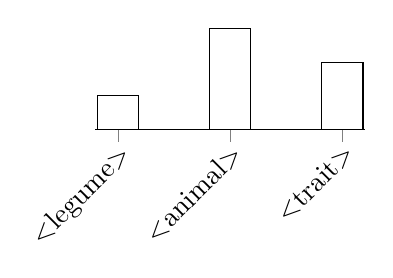
\begin{tikzpicture}
    \begin{axis}[
        ybar=1pt,
        bar width=15pt,
        ymin=0,
        width=5cm,
        height=3cm,
     hide y axis,
     axis x line*=bottom,
        symbolic x coords={$<$legume$>$, $<$animal$>$, $<$trait$>$},
        xtick = data,
        x tick label style={rotate=45, anchor=north east, inner sep=0mm},
        legend pos=north west
    ]
    \addplot[fill=none] coordinates {($<$legume$>$, 1) ($<$animal$>$, 3) ($<$trait$>$, 2)};
    \end{axis}
\end{tikzpicture}
\hspace{1cm}
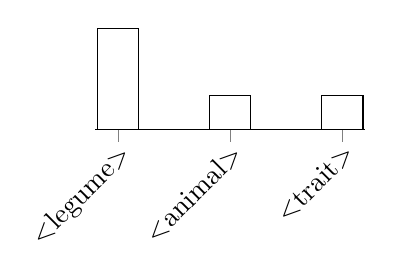
\begin{tikzpicture}
    \begin{axis}[
        ybar=1pt,
        bar width=15pt,
        ymin=0,
        width=5cm,
        height=3cm,
     hide y axis,
     axis x line*=bottom,
        symbolic x coords={$<$legume$>$, $<$animal$>$, $<$trait$>$},
        xtick = data,
        x tick label style={rotate=45, anchor=north east, inner sep=0mm},
        legend pos=north west
    ]
    \addplot[fill=none] coordinates {($<$legume$>$, 3) ($<$animal$>$, 1) ($<$trait$>$, 1)};
    \end{axis}
\end{tikzpicture}
\end{figure}
\end{center}

Under this view, selectional preferences are fully encoded by the change between the prior and the posterior distribution. Resnik implemented this intuition with his Selectional Preference Strength (SPS) measure, defined as the Kullback-Leibler divergence (relative entropy) between the two distributions, as in \refeq{resnik_sps_eq}.

\begin{equation} \labeq{resnik_sps_eq}
SPS_{v,r} = \sum_{c \in classes} p(c|v,r) \: \log_{2}\frac{p(c|v,r)}{p(c|r)}
\end{equation}

In \refeq{resnik_sps_eq}, $p(c|v,r)$ is the posterior distribution of argument classes for a given predicate $v$ in a given relation $r$ with the predicate, and $p(c|r)$ is the prior distribution of argument classes regardless of the predicate. The only relevant relation for the purposes of this thesis is the verb-object relation, but it can also be any other grammatical function (such as verb-subject) or semantic role (such as verb-Instrument, as in \textcite{CappelliLenciPISA}). Given a set of transitive verbs used in a corpus, SPS scores will be higher for transitive verbs having a narrow selectional range (as in \ref{dobj1}) and lower for those having a broader selectional range (as in \ref{dobj2}).
\ex.\label{ex1} \a. \label{dobj1} John ate $\varnothing$\textsubscript{object}.
\b. \label{dobj2} *John made $\varnothing$\textsubscript{object}.

Crucially, selectional preferences as measured by SPS provide insight about the recoverability of direct objects, and their recoverability affects the grammaticality of the sentences in \ref{ex1}. In particular, \textit{to eat} selects mostly for edible items, so that reading \ref{dobj1} we can reasonably assume John ate some kind of food, while \textit{to make} selects for a wide array of objects from semantically different classes, so it's impossible to know what is that John made in \ref{dobj2}.\\
The classes considered when computing the SPS scores have to belong to a lexical taxonomy, so that each sense of each noun in the lexicon is mapped to a concept. Using Resnik's example \parencite[59]{Resnik1993}, the noun \textit{baseball} can be mapped to two concepts, i.e. a hyponym of the concept $<$ball$>$ and a hyponym of the concept $<$field game$>$. Moving from concepts to taxonomy classes, a noun belongs to any class having one of its concepts as a hyponym, even indirectly. Thus, as illustrated in \reffig{wordnet_simplified}, \textit{baseball} belongs not only to the classes $<$ball$>$ and $<$field game$>$, but also to $<$game equipment$>$, $<$artifact$>$, $<$inanimate object$>$, $<$outdoor game$>$, $<$sport$>$, $<$human activity$>$, and $<$entity$>$ (the root node of the whole hierarchy).

\begin{figure}[htb]
\caption{Simplified representation of the noun \textit{baseball} in the lexical taxonomy.}
\labfig{wordnet_simplified}
\centering
\begin{forest}
[$<$entity$>$
  [$<$inanimate object$>$
    [$<$artifact$>$
      [$<$game equipment$>$
        [$<$ball$>$,name=S1 [\textit{baseball},phantom]
        [...,tier=mytier]
        [...,tier=mytier]
        [...,tier=mytier]
        ] 
  [...
  ]
      ]
  [...
  ]
    ]
  [...
  ]
  ]
  [\textit{baseball},tier=mytier,no edge,name=shared]
  [...
  ]
  [$<$human activity$>$
    [$<$sport$>$
        [$<$outdoor game$>$
            [$<$field game$>$,name=S2 [\textit{baseball},phantom]
        [...,tier=mytier]
        [...,tier=mytier]
        [...,tier=mytier]
            ]
  [...
  ]
        ]
  [...
  ]
    ]
  [...
  ]
  ]
]
\draw (S2) -- (shared);
\draw (S1) -- (shared);
\end{forest}
\end{figure}

In order to compute SPS scores, Resnik adopts WordNet \parencite{beckwith1991wordnet,Miller1995} as a computational model of the lexical taxonomy. Its appeal to the author \parencite[32]{Resnik1993} lies in that the WordNet taxonomy encodes knowledge in an explicit, hierarchical fashion, which is "intuitively reasonable" and "widely accepted".\\ While powerful in many respects, Resnik's model of selectional preferences has a crucial drawback, which is the need for a manually-built lexicon. This requirement makes it difficult to compute SPS scores for verbs in languages without a WordNet, for neologisms, and for special registers not yet encoded in WordNet. Given this severe limitation, I decided \hl{to improve on} Resnik's SPS to model the recoverability of direct objects, creating a model based on distributional semantics \parencite{Lenci:2018} that can be applied in all the cases where the SPS measure cannot.

\paragraph{Results}
The SPS scores for the English and Italian transitive verbs under consideration are fully listed in \refappsec{app_resnik}.\\ % \vspace{}

\subsection{Computational PISA}\labsec{compuPisa}

Distributional semantics is based on the Distributional Hypothesis, which states that words occurring in the same contexts tend to have similar meanings, or, quoting the popular formula from \textcite{firth1957synopsis}, that "you shall know a word by the company it keeps". Such a framework puts the meaning of words in the ever-changing use speakers make of language, instead of securing it in the nodes of a static lexical taxonomy. Most importantly, distributional semantics posits a correlation between distributional similarity and semantic similarity and uses the former to model the latter. Roughly, the semantic space where words "keep company" can be modeled as a vector space where each word is a vector whose dimensions are context words. An example is provided in \reffig{vectorspace}, where the two words \textit{hamburger} and \textit{dragon} populate a semantic space defined by the three context words \textit{big}, \textit{tasty}, and \textit{mythological}. The coordinates of \textit{hamburger} are (2,2,0) because in this hypothetical situation it occurs twice with \textit{big}, twice with \textit{tasty}, and never with \textit{mythological}, while the coordinates of \textit{dragon} are (2,0,1) because it occurs twice with \textit{big}, never with \textit{tasty}, and once with \textit{mythological} in the hypothetical corpus.

\begin{figure}[htb]
\caption{Simplified representation of the words \textit{hamburger} and \textit{dragon} in a vector space.}
\labfig{vectorspace}
\centering
\begin{tikzpicture}[x=1cm, y=1cm, z=-0.6cm]
    % Axes
    \draw [->] (0,0,0) -- (4,0,0) node [right] {$big$};
    \draw [->] (0,0,0) -- (0,4,0) node [left] {$tasty$};
    \draw [->] (0,0,0) -- (0,0,4) node [left] {$mythological$};
    % Vectors
    \draw [->, thick] (0,0,0) -- (2,2,0);
    \draw [->, thick] (0,0,0) -- (2,0,1);
    % Ticks
        \foreach \i in {1,2}
    {
    \draw (-0.1,\i,0) -- ++ (0.2,0,0);
    \draw (\i,-0.1,0) -- ++ (0,0.2,0);
    \draw (-0.1,0,\i) -- ++ (0.2,0,0);
    }
    % Dashed lines
    \draw [loosely dashed]
        (0,2,0) -- (2,2,0) -- (2,0,0)
        (0,0,1) -- (2,0,1) -- (2,0,0)
        ;
    % Labels
     \node [right] at (2,2,0) {hamburger};
   \node [below] at (2,0,1) {dragon};

\end{tikzpicture}
\end{figure}

How does all of this translate into a solution to the problem of having a taxonomy-free model of argument recoverability? Let us go back to the example in \ref{ex1} and consider the distribution of the arguments of the two verbs \textit{to eat} and \textit{to make} in a corpus. Ideally, collapsing on a 2-dimensional grid the $n$-dimensional space populated by these arguments, the distribution of the arguments of \textit{to eat} would resemble \reffig{mock_args_eat} and the distribution of the arguments of \textit{to make} would resemble \reffig{mock_args_make}. The (recoverable) arguments of \textit{to eat} are close together in the vector space, while the (non-recoverable) arguments of \textit{to make} are very sparse in the same space.

\begin{figure}[htb]
\caption{Made-up representation of the possible distribution of the direct objects of the verb \textit{to eat} in a vector space.}
\labfig{mock_args_eat}
\centering
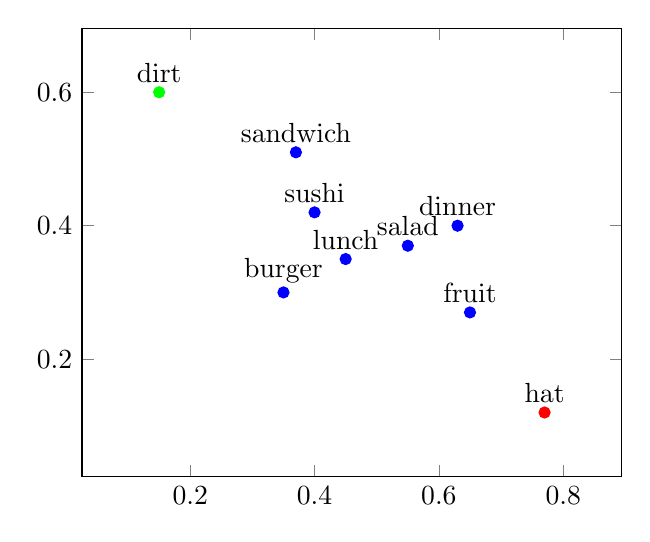
\begin{tikzpicture}
\begin{axis}[enlargelimits=0.2]
    \addplot[
        scatter/classes={a={blue}, b={red}, c={green}},
        scatter, mark=*, only marks, 
        scatter src=explicit symbolic,
        nodes near coords*={\Label},
        visualization depends on={value \thisrow{label} \as \Label} %<- added value
    ] table [meta=class] {
        x y class label
        0.63 0.4 a dinner
        0.45 0.35 a lunch
        0.4 0.42 a sushi
        0.55 0.37 a salad
        0.37 0.51 a sandwich
        0.35 0.3 a burger
        0.65 0.27 a fruit
        0.77 0.12 b hat
        0.15 0.6 c dirt
    };
\end{axis}
\end{tikzpicture}
\end{figure}

\begin{figure}[htb]
\caption{Made-up representation of the possible distribution of the direct objects of the verb \textit{to make} in a vector space.}
\labfig{mock_args_make}
\centering
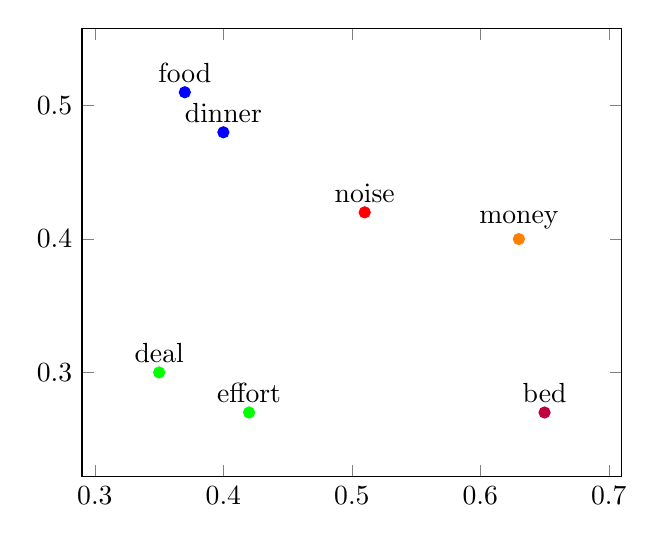
\begin{tikzpicture}
\begin{axis}[enlargelimits=0.2]
    \addplot[
        scatter/classes={a={blue}, b={red}, c={green}, d={orange}, e={purple}},
        scatter, mark=*, only marks, 
        scatter src=explicit symbolic,
        nodes near coords*={\Label},
        visualization depends on={value \thisrow{label} \as \Label} %<- added value
    ] table [meta=class] {
        x y class label
        0.37 0.51 a food
        0.4 0.48 a dinner
        0.63 0.4 d money
        0.51 0.42 b noise
        0.42 0.27 c effort
        0.35 0.3 c deal
        0.65 0.27 e bed
    };
\end{axis}
\end{tikzpicture}
\end{figure}

Based on these consideration, the conclusion is that the closer the direct objects of a verb are in a vector space, the more recoverable they should be. This is the main intuition behind Computational PISA, whose computational implementation I will discuss in the next paragraph.

\paragraph{Computational implementation} Computational PISA is defined as the semantic density of a verb-relation pair, i.e. the mean value of the pairwise cosine similarity between the arguments of the pair. In this thesis, this means calculating the mean pairwise cosine similarity between all the direct objects of a given transitive verb. \hl{The full script used to obtain Computational PISA scores using a corpus and a list of verbs as input is available} \href{http://www.overleaf.com}{on GitHub}. \\
This is done in two steps, for each transitive verb under consideration. The first one is to compute the Selectional Association between the verb and each one of its direct objects as defined by \textcite{Erk2007, ErkEtAl2010} in \refeq{erkpadopado}. This is a measure of the strength of the selectional preference \textit{SA} of a verb for a possible argument \textit{a\textsubscript{0}}, modeled as the weighted sum of the similarities between the candidate argument \textit{a\textsubscript{0}} and the actual arguments found in the corpus (each called \textit{a} in the formula). In \textcite{CappelliLenciPISA} and this dissertation I measure argument similarity with the cosine similarity.

\begin{equation} \labeq{erkpadopado}
SA_{v,r} (a_0) = \sum_{a \in args(v,r)} wt_{v,r}(a) \: sim(a_0,a)
\end{equation}

Then, Computational PISA scores are computed as in \refeq{pisa}, i.e. by averaging \refeq{erkpadopado} over the \textit{n} direct objects of a given transitive verb.

\begin{equation} \labeq{pisa}
PISA_{v,r} = \frac{1}{n} \sum_{i = 1}^{n} SA_{v,r} (a_i)
\end{equation}

In \textcite{CappelliLenciPISA} five weight functions are used to compute \refeq{erkpadopado} and then \refeq{pisa} (\refeq{uni}, \refeq{freq}, and \refeq{idf} are taken from \textcite{ErkEtAl2010}). In detail, the functions are as follows.
\begin{itemize}

\item \textbf{UNI} assumes a uniform distribution. This actually yields an \textit{un}weighted model, because in \refeq{erkpadopado} the argument similarity is always multiplied by 1.
\begin{equation} \labeq{uni}
wt_{v,r}(a) = 1
\end{equation}

\item \textbf{FRQ} is the co-occurrence frequency of a given direct object with the transitive verb under consideration.
\begin{equation} \labeq{freq}
wt_{v,r}(a) = freq(a,v,r)
\end{equation}

\item \textbf{IDF} is inspired to the well-known Inverse Document Frequency weighting scheme, which
assigns higher scores to direct objects occurring with fewer transitive verbs (the minimum would be 0, for an argument that occurs with every verb in the corpus). This is done in order to mitigate the frequency effect of arguments occurring with too many verbs to be considered relevant for the specific target verb under examination. In \refeq{idf}, $|v,r|$ is the number of transitive verbs in the corpus, and $|v,r : a \in v,r|$ is the number of transitive verbs having $a$ as a direct object.
 \begin{equation} \labeq{idf}
wt_{v,r}(a) = \log _{} \frac{|v,r|}{|v,r : a \in v,r|}
\end{equation}

\item \textbf{LMI} is the Local Mutual Information \parencite[89]{evert2005statistics-lmi} of the direct object and a given transitive verb, computed as in \refeq{lmi}. The LMI compares the probability of a noun occurring in a corpus as the direct object of a verb with the probability of the noun and the transitive verb occurring in a corpus without any relation to one another. In other words, given a noun and a transitive verb, their LMI is computed as the logarithmic ratio of their joint probability and the product of their individual probabilities in the corpus (i.e. their joint probability if they were statistically independent events).
 \begin{equation} \labeq{lmi}
wt_{v,r}(a) = f(a,v,r) \log _{2} \frac{p(a,v,r)}{p(a)p(v,r)}
\end{equation}  

\item \textbf{ENT} is the entropy \parencite{shannon1948mathematical} of the direct objects of a given transitive verb. Information theory uses entropy to quantify the informativity of a given event, inheriting its mathematical definition from thermodynamics. The entropy of an event (which in \refeq{ent} is the argument itself) is a function whose value decreases as the probability of the event increases.
 \begin{equation} \labeq{ent}
wt_{v,r}(a) = -\!\sum_{\mathclap{a \in args(v,r)}} p(a) \log _{2}p(a)
\end{equation}
In \refeq{ent}, $p(a) = \frac{f(a)}{\sum_{a_0 \in A}f(a_0)}$, where $A$ is the complete set of the direct objects of the target verbs, extracted from the corpus.
\end{itemize}

\paragraph{The original experiment}
In \textcite{CappelliLenciPISA}, I computed weighted models of argument recoverability, as explained in the previous paragraph, and also unweighted models, only taking into account 300 direct objects for each transitive verb. For each verb, the relevant 300 objects were selected after sorting the entire list of direct objects based on the FRQ, IDF, LMI and ENT functions. The reason to include unweighted models in the experiment stems from the observation that the computation of \refeq{pisa} for verbs with a large number of direct objects can get cumbersome, and it may be possible to achieve a comparable degree of informativity by only considering the most relevant objects occurring with each verb.\\
I tested the models on a 99-verb set of transitive verbs, extracting their direct objects from ukWaC, a 2-billion token part-of-speech tagged and lemmatized corpus of English \parencite{FerraresiEtAl2008}. Direct objects were modeled as bare head nouns, excluding any determiner and modifier present in the DP (e.g. \textit{sword} instead of \textit{a big rusty sword}). I obtained the vector representation of direct objects by using 12 different 300-dimensional embeddings trained on a concatenation of ukWaC and a 2018-dump of English Wikipedia, including both SVD-reduced count-based DSMs and neural embeddings.\\
Since Computational PISA was intended to model argument recoverability, I tested the results of each model by means of a Mann-Whitney U test comparing the mean Computational PISA score of the recoverable-object transitive verbs with the mean Computational PISA score of the non-recoverable-object transitive verbs. Summing up the discussion of the results carried out in the original paper (here in \reftab{tab:mwu}), it was found that the weighted versions of Computational PISA yield highly significant results, while the unweighted versions yield results with a comparable degree of significance just with the FRQ sorting function and, in particular, running the model on word2vec \parencite{mikolov2013efficient} distributional spaces.

\begin{table}
\caption{Mann-Whitney U tests comparing recoverable- and non-recoverable-argument verbs (significance levels).}
\labtab{tab:mwu}
\centering
\begin{small}
\begin{tabular}{llccc}
\hline & & \textbf{weighted} & \textbf{top $k$} & \textbf{bot $k$} \\ \hline
 & SVD & *** & - & - \\
\texttt{\textbf{UNI}} & w2v & *** & - & - \\
 & w2vf & ** & - & - \\
 \hline
 & SVD & *** & ** & ns \\
\texttt{\textbf{FRQ}} & w2v & *** & *** & ns \\
 & w2vf & *** & ** & ns \\
 \hline
 & SVD & *** & ** & ns \\
\texttt{\textbf{IDF}} & w2v & *** & *** & *** \\
 & w2vf & ** & ns & ns \\
 \hline
 & SVD & *** & ** & ns \\
\texttt{\textbf{LMI}} & w2v & *** & * & * \\
 & w2vf & *** & * & * \\
 \hline
 & SVD & *** & ns & ns \\
\texttt{\textbf{ENT}} & w2v & *** & *** & ns \\
 & w2vf & *** & * & * \\
\hline
\end{tabular}
\end{small}
\end{table}

\paragraph{\hl{Operative choices}}
Drawing from the results discussed in \textcite{CappelliLenciPISA} and summarized in the previous paragraph, I computed Computational PISA scores for my verbs of interest in English and Italian. For English, I based the calculations on ukWaC as in the original study, and for Italian, I based them on itWaC, a 2-billion token part-of-speech tagged and lemmatized corpus of Italian \parencite{baroni2009wacky}. Given that web-scraped, automatically tagged corpora this large inevitably suffer from significant noise in the data, which then results in possibly unreliable results, I pre-processed the data extracted from both corpora to minimize the impact of noise and tagging mishaps. First of all, I filtered the 65,000 direct objects of my 30+30 verbs of interest so that they were:
\begin{itemize}
    \item not hapaxes (considering the verb-noun frequencies)
    \item having an absolute frequency in the corpus greater than 100
    \item present in WordNet (to eliminate misspelled words)
\end{itemize}
Then, I manually filtered the remaining nouns so that each verb only takes direct objects which do not belong to any of these categories:
\begin{itemize}
    \item idiomatic senses (e.g. 'ice' as an object of 'to break')
    \item metaphoric senses (e.g. 'mind' as an object of 'to poison')
    \item direct objects of an unintended meaning of the verb (e.g. 'salmon' as an object of 'to smoke', since the intended sense of 'to smoke' in my study is only the one related to inhaling the byproduct of the combustion of tobacco and other plants)
    \item unintended direct objects (e.g. Recipients in double-object constructions such as 'pupils' in 'to teach pupils Linguistics', since in my study I am only interested in Theme/Patient direct objects)
    \item mistagged direct objects (e.g. 'disorder' as an object of 'to eat', which is clearly the result of the automatic corpus tagger interpreting 'eating' in 'eating disorder' as a verb rather than as an adjective)
    \item 'thing' (and 'stuff'), which appears with every transitive verb and is thus irrelevant
\end{itemize}
The files containing the complete list of direct objects of each verb, both raw and cleaned, both in English and in Italian, are freely available \href{https://github.com/giuliacappelli/dissertationData}{on my GitHub profile}.\\
Based on the results from the original Computational PISA study, I based my computations on word2vec neural embeddings (which yield consistently reliable results) and employed the FRQ weighting funtion (which is the best-performing among all five, both in weighted and in sorted models of Computational PISA).

\paragraph{Results}
The Computational PISA scores for the English and Italian transitive verbs under consideration are fully listed in \refappsec{app_cpisa}.\\ % \vspace{}


\subsection{\hl{Behavioral PISA}}\labsec{behavPisa}

\paragraph{Introduction} 
Despite representing a clear step forward compared to Resnik's taxonomy-based measure of selectional preferences, a corpus-based measure such as Computational PISA still has notable downsides. First of all, the corpus on which Computational PISA calculations are based has to be large enough to feature all the verbs under consideration, and for each verb to present a sufficient number of direct objects to allow for the computation of meaningful Computational PISA. It may well be the case that using a small corpus forces an experimenter to draw from a different set of verbs than intended for their study, if not all of them are featured in the corpus. Moreover, low-frequency verbs may appear with a small set of direct objects even in large corpora, making it potentially difficult to obtain reliable Computational PISA scores. Another order of problems (which larger, automatically-tagged corpora are more prone to suffer from than smaller, manually-tagged ones) depends on noisy or otherwise inaccurate corpus data. For instance, large corpora constructed via crawling the Web (such as ukWaC and itWaC) typically present a substantial number of misspelled words and mis-tagged parts of speech, making it necessary to clean them manually beforehand. In addition to this, even clean corpora often lack fine-grained semantic information, about thematic roles (e.g. distinguishing the Theme and the Recipient in 'John gave Mary a book'), polysemy (e.g. 'to graduate' may mean 'to become a doctor', but also 'to arrange something in gradations'), idiomatic uses of verbs (e.g. there is usually no actual bucket being kicked when someone 'kicks the bucket').\\
In order to overcome these problems and obtain equally reliable scores for each verb in my experiment, I decided to implement a behavioral variant of the original Computational PISA measure. In the case of Behavioral PISA, the semantic similarity of a given verb's direct objects is not approximated via their distributional similarity in a corpus, but instead via their psychological similarity as judged by native speakers of the languages under study. Such a measure is intended to provide robust data for each verb regardless of its corpus frequency or scarcity of direct objects with respect to other verbs, at the cost of having to perform a behavioral experiment with human subjects.

\paragraph{Experimental protocol}
The experimental procedure to obtain the relevant data and compute the Behavioral PISA scores follows closely the method Medina used in her thesis to compute a comparable measure, which she calls "Object Similarity" \parencite[173-178]{Medina2007}, and whose purpose is to overcome the shortcomings of Resnik's SPS. In a sense, Object Similarity may be viewed as a behavioral precursor of Computational PISA, both being based on a broad notion of selectivity-as-semantic-closeness.\\
In order to build the stimuli, I picked 6 pairs of direct objects for each verb of interest in my two 30-verb sets (one for English and one for Italian, as detailed in \nrefch{judgments}). For each verb, the direct objects comprising the 6 pairs were randomly selected from the manually cleaned (see \nrefsec{compuPisa}) verb-object lists, so that each pair contained two different direct objects. This operation resulted in 180 stimuli (30 verbs x 6 direct objects) for each language, which the interested reader will find in \refapp{app_behavPisa}. Each pair of direct objects works as a stimulus, without explicit mention of the verb which subcategorizes the objects in the pair.\\
The two lists of 180 stimuli was used to create two Google Form surveys (with randomized stimuli), and 25 unpaid raters were recruited online for each language among native speakers holding at least a Bachelor's degree. Each rater had to judge the similarity of the two objects in each pair on a 7-point Likert scale in a single experimental session. Crucially, the participants to the experiment were not provided with a strict definition of similarity, and they did not know that the stimuli were direct objects of a given set of verbs. Instead, they were told that the pair 'love - upholstery' should get a rating of 1 an the pair 'cat - dog' should get a rating of 7, to familiarize them with the Likert scale, and they were encouraged to make use of the whole 7-point scale whenever necessary.

\paragraph{Computational implementation} Behavioral PISA is defined as the mean pairwise similarity between a subset of direct objects of a transitive verb. The pairwise similarity is obtained via human similarity judgments on a 7-point Likert scale, as described right above. In order to account for individual differences in the use of the scale, I computed the within-subject z-scores of these results, and then I averaged the normalized scores to obtain a single value for each verb of interest \parencite{KimEtAl2018, KimEtAl2019, KimEtAl2019a} as in \refeq{eq_behavPisa}, where $r$ is a (normalized) rating and $i$ is the total number of ratings.

\begin{equation} \labeq{eq_behavPisa}
PISA_{v} = \frac{\sum_{i} r_{v}}{i}
\end{equation}

The Behavioral PISA scores thus obtained were then normalized to fall between 0 and 1. The Python script I coded to generate the stimuli and compute the Behavioral PISA scores for each verb is freely available \href{https://github.com/giuliacappelli/behavioralPISA}{on my GitHub profile}.

\paragraph{Results} 
The Behavioral PISA scores for the English and Italian transitive verbs under consideration are fully listed in \refappsec{app_bpisa}.\\ 

\section{Telicity} \labsec{predictor_telicity}

% Most importantly, under the definition of telicity as a privative opposition by \textcite[33]{Olsen1997telicity-privative} (implemented in the Stochastic Optimality Theoretic model of object omissibility by \textcite{Medina2007}), "no constituent may cancel the marked interpretation: [+telic] verbs are always interpreted as having an inherent end", while "atelicity is a cancelable conversational implicature".\\

\subsection{Telicity tests}
\nrefsec{telicity} introduced telicity as a major predictor of object omissibility. Since aspectual interpretation is compositional \parencite[14]{Olsen1997}, a transitive verb which can be used both transitively and intransitively tends to get a telic interpretation in the first case and an atelic interpretation in the second case.\\ 
In my behavioral experiments and subsequent linguistic models of object drop, I operationalize telicity as a binary feature, based on theoretical claims discussed before. A verb is considered [+Telic] if two tests yield a telic interpretation, [-Telic] otherwise. Out of Medina's set, I only used the staple \textit{in/for} test for telicity, rejecting the \textit{almost} test since it is notoriously quite problematic with achievements (please refer to \textcite{bertinetto-delfitto2000aspect} for an extensive discussion on the issue).\\
Verbs were tested without a direct object to avoid involuntarily eliciting a telic interpretation, or with a generic object (e.g. "something") if the intransitive use yields a grammatically unacceptable interpretation. The two tests used for the experiments of this thesis are as follows (the reader is referred to \textcite{Borik2006} and \textcite{Liu2014} for a detailed review of telicity tests)\sidenote{I also considered the \textit{conjunction} test for telicity, but then decided to discard it because it is weaker than the other two. This diagnostic requires that the predicate be tested in a sentence where it it modified by two conjoined temporal adjuncts denoting consecutive time slots, as in \ref{conj_test}. Telic verbs in this construction, as in \ref{conj_telic}, imply two separate events (i.e. John built something on Saturday and something else on Sunday). On the contrary, sentences with atelic verbs, as \ref{conj_atelic}, can be interpreted either as two separate events (i.e. John sang on Saturday, stopped, and resumed his singing on Sunday) or as a continuous event (John sang on both days without interruption).
\ex.\label{conj_test} \a. John built something on Saturday and on Sunday. \label{conj_telic} 
\b. John sang on Saturday and on Sunday. \label{conj_atelic}}.

\paragraph{\textit{In/for} test} Based on this largely agreed-upon diagnostic for telicity, telic predicates (e.g. \textit{build} in \ref{infor_telic}) are only grammatical if used with time-frame adverbials such as "in X time", while atelic predicates (e.g. \textit{sing} in \ref{infor_atelic}) are grammatical if used with time-span adverbials such as "for X time".
\ex. \label{infor_telic} \a. John built something in an hour.
\b. \%John built something for an hour.

\ex. \label{infor_atelic} \a. *John sang in an hour.
\b. John sang for an hour.

\paragraph{\textit{Progressive} entailment test} The progressive form of a predicate bears different pragmatic implicatures based on whether it is telic or atelic. In particular, saying that the subject "was \textit{verb}ing" implies that they \textit{verb}ed with atelic verbs as in \ref{progressive_atelic}, while this is not true for telic verbs as in \ref{progressive_telic}.
\ex. \a. John was building something. \label{progressive_telic} 
\b. John was singing. \label{progressive_atelic}

\subsection{Results}
The telicity features of each English and Italian transitive verb are listed in \refappsec{app_telicity}.



\section{Perfectivity} \labsec{predictor_perfectivity}

Perfectivity is discussed at large as a possible determinant of object drop in \nrefsec{perfectivity}. The main point is that transitive verbs resist the omission of their direct object when used in the perfective aspect (as in \ref{perf_ex1}), while verbs in the imperfective aspect are much more likely to allow it (as in \ref{perf_ex2}).
\ex.\label{perf_ex} \a. ? John painted. \label{perf_ex1} 
\b. John was painting. \label{perf_ex2}

Like telicity, perfectivity appears as a binary feature in my experiments and models. Unlike telicity, perfectivity is not an inherent feature of verbs, so it cannot be tested beforehand: instead, I will include it in the behavioral experiments by having both perfective and imperfective uses of the same verb (please refer to \nrefch{judgments} for a complete overview of the experimental design). The reader will find the results of these operative choices in \refapp{app_stimuli}.

\subsection{A note on tense}
To choose the correct tenses to encode (im)perfectivity in English and in Italian, a critical discussion on the relation between tense and aspect is in order. A common perspective on grammatical aspect in English, as summarized by \textcite[106]{smith1991parameter} and \textcite[663]{wagner2001aspectual}, is that perfective aspect corresponds to the simple form of the verb, while the imperfective aspect is derived by means of the progressive construction (i.e. by adding the auxiliary \textit{be} and \textit{-ing} to the main verb). This perspective has the undeniable merit of keeping grammatical aspect and lexical aspect apart, acknowledging the orthogonality of (a)telicity and (im)perfectivity (refer to \textcite{bertinetto2001frequent} for an extensive discussion on the issue). However, the view that the simple form of a verb is necessarily interpreted as perfective has long since been abandoned.\\
Based on \textcite{Olsen1997, bertinetto2001frequent}, the simple past in English is not marked for the perspective aspect. On the contrary, simple verb forms are aspectually unmarked, and they get different aspectual interpretations based on the interaction of tense, lexical aspect, and the different context they appear in. For this reason, for the experimental stimuli I will choose tenses that are aspectually marked, as to avoid misinterpretations.\\
Even though simple past does not equate to perfective aspect, it's true that past tense hints towards perfectivity, as noted by \textcite{comrie1976aspect} and later on by \textcite{wagner2001aspectual, Olsen1997, Medina2007}, among others. So, a morphologically unmarked past form is more likely to be interpreted as perfective than a non-past form. Moreover, there are differences internal to the group of past forms. In fact, as we saw before, the simple past is aspectually unmarked, but the past perfect (e.g. \textit{John had written a book.)} is marked as perfective.

\subsection{Operative choices}
Considering what has been noted in the previous paragraph, and following \textcite{Medina2007}, in the experimental stimuli perfective aspect will be encoded with perfect morphology and imperfective aspect will be encoded with progressive morphology.\\
For English, perfective stimuli will be in the past perfect tense (as in \ref{perf_ex1_eng}) and imperfective stimuli in the past continuous tense (as in \ref{perf_ex2_eng}). For Italian, perfective stimuli will be in the \textit{\hl{tra}passato prossimo} tense (as in \ref{perf_ex1_ita}) and imperfective stimuli in the continuous past form created with the auxiliary 'to stay' in the \textit{imperfetto} tense and the simple gerund of the main verb (as in \ref{perf_ex2_ita}). 
\ex.\label{perf_ex_eng} \a. John had played. \label{perf_ex1_eng} 
\b. John was playing. \label{perf_ex2_eng}

\ex.\label{perf_ex_ita} \a. Gianni \hl{aveva} cantato. \label{perf_ex1_ita} 
\b. Gianni stava cantando. \label{perf_ex2_ita}

On a side note, Italian also has perfective-only and imperfective-only simple past tenses, namely \textit{passato remoto} and \textit{imperfetto}, but I chose to use compound tenses since \textit{passato remoto} lost some ground to \textit{passato prossimo} over the last few decades, and also considering the variety of regional uses of \textit{passato remoto} \parencite{bertinetto1996distribuzione}. \hl{Most importantly, the \textit{trapassato} \textit{prossimo} tense was chosen to encode perfective aspect in Italian because it's the aspectually closest Italian tense to the English past perfect, despite the glaring differences between the aspectual systems in these two languages (Bertinetto 1992)}.

% QUI DEVO CITARE \parencite{bertinetto1992piucheperf}, CHE PER QUALCHE MOTIVO CREA ERRORI ANCHE SE FORMALMENTE SEMBRA CORRETTO

% Il mio suggerimento di rifare l'esperimento nasce dal fatto che occorre sempre confrontare (nei limiti del possibile) gli stessi oggetti. Questo principio viene violato se si confrontano piucheperfetto da un lato, e passato 'prossimo' dall'altro.

\section{Iterativity} \labsec{predictor_iterativity}

As argued in \nrefsec{iterativity}, iterativity and other types of pluractionality favor the omission of direct objects (compare \ref{iterat_ex1} and \ref{iterat_ex2}). Although well-known in the theoretical literature \parencite{Glass2013, Glass2020, Ruda2017}, to my knowledge this predictor of object drop appears here for the first time in a comprehensive linguistic model based on acceptability judgments.
\ex.\label{iterat_ex} \a. \# The Joker killed. \label{iterat_ex1} 
\b. The Joker killed again. \label{iterat_ex2}

Iterativity is yet another binary predictor and it will be encoded in the behavioral experiments in the same way as perfectivity, that is to say, by creating both iterative and non-iterative stimuli for the same verb as in \ref{iterat_ex} (please refer to \refapp{app_stimuli} for the complete set).

\section{Manner specification} \labsec{predictor_mannspec}

The effects of manner specification on indefinite object drop are presented in \nrefsec{mannerspec}. As argued by \textcite{Ruda2017} a.o., if a transitive verb allows for its direct object to be dropped, then its synonyms with a specific manner component block it. This is evident in \ref{mannspec_ex}: the base verb \textit{to eat} allows for object drop in \ref{mannspec_ex1}, but its manner-specified counterparts \textit{to devour/nibble/chew} in \ref{mannspec_ex2} do not.
\ex.\label{mannspec_ex} \a. John ate. \label{mannspec_ex1} 
\b. * John devoured/nibbled/chewed. \label{mannspec_ex2}

In the following experiments, manner specification is treated as a binary predictor. The verbs used in the stimuli are marked in \refapp{app_predictors} as either manner specified or manner unspecified. Just as in \ref{mannspec_ex}, verbs tagged as manner specified are marked counterparts of manner unspecified verbs present in the list, to make the experimental design and subsequent modeling more robust.
